In order to maximize the sensitivity to the signal models of Figure~\ref{fig:strategy.pheno.feynman}, 13 non-exclusive signal regions are defined in Table~\ref{tab:SRdef3}. 
The SRs are named in the form \textit{RPCN}L{\textit M}b{\textit X}, where {\textit N} indicates the number of leptons required, {\textit M} the number of $b$-jets required, and {\textit X} indicates the severity 
of the \met or \meff\ requirements (Soft, Medium or Hard). All signal regions allow any number of additional leptons in addition to a $e^\pm e^\pm$,
$e^\pm \mu^\pm$ or $\mu^\pm \mu^\pm$ pair. Signal regions with 3 leptons can be either any charge combination or all three with the same charge (Rpc3LSS1b).
For each lepton/$b$-jet multiplicity, two signal regions are defined targeting either compressed spectra or large mass splittings. 

The optimization of the definitions of signal regions relied on a brute-force
scan of several discriminating variables in a loose classification of events 
in terms of number of $b$-jets and/or leptons in the final state, each being 
associated to the signal scenario favouring this final state.
The other main discriminant variables (e.g number of jets above a certain \pt threshold, \meff, \met, $\met/\meff$ ratio) were then allowed to vary, 
to determine for each point of the parameter space the best configuration. 
The figure of merit used to rank configurations was the discovery significance 
for a statistical test based on a ratio of two Poisson means~\cite{Cousins:2009}.
A realistic systematic uncertainty of $30\%$ on the expected background yield 
was included in the statistical test.
To preserve the discovery potential, only configurations leading to at least two signal events were considered for a given signal point. The total number of background events should not be smaller than 1; to model in a more realistic way the effect of non-prompt and fake leptons and electron charge mis-identification backgrounds, 
which are determined from data in the analysis, 
the MC predictions for those processes in $\ttbar$ and $Z$+jets MC were scaled 
using the factors obtained from the MC template method (Section~\ref{sec:fake.mct}), as shown in Table~\ref{tab:mctemplateF}.
Note that different corrections are applied depending on the showering (Pythia or Sherpa) used for each sample, 
and for the fake and non-prompt leptons originated from heavy-flavour (HF) and light-flavour (LF).

\begin{table}[!htb]
\caption{Scaling factors applied to the electron charge-flip and non-prompt/fake lepton background in the SR optimization procedure.}
\label{tab:mctemplateF}
\def\arraystretch{1.1}
\centering
\begin{tabular}{|c||c|c|c|c|c|}
\hline 
& Charge mis-id & HF $e$ & HF $\mu$ & LF $e$ & LF $\mu$ \\ \hline\hline
Pythia & 0.96 $\pm$ 0.08 & 1.80 $\pm$ 0.45 & 2.10 $\pm$ 0.58 & 1.55 $\pm$ 0.14 & 0.74 $\pm$ 0.81\\\hline
Sherpa & 1.02 $\pm$ 0.09 & 2.72 $\pm$ 0.57 & 1.81 $\pm$ 0.75 & 1.16 $\pm$ 0.18 & 1.84 $\pm$ 1.16\\
\hline
\end{tabular}
\end{table}


\begin{table}[tbh!]
%\rotatebox{90}
\centering
\resizebox{\textwidth}{!}
{
\hspace{0.5cm}
\def\arraystretch{1.2}
\small
\begin{tabular}{|l|c|c|c|c|c|r|c|c|l|}
\hline
Signal region  &  $N_{\textrm{leptons}}^{\textrm{signal}}$   & $N_{b\textrm{-jets}}$ & $N_{\textrm{jets}}$  & $\pt^{\textrm{jet}}$ & \met\ & \meff\ & \met/\meff  & Other & Targeted  \\
               &                                  &                   &                  &    [GeV]             & [GeV] & [GeV] &   &  & Signal  \\
\hline\hline

Rpc2L2bS         & $\ge 2$SS  & $\ge 2$ & $\ge 6$ & $>25$ & $>200$ & $>600$  & $>0.25$    & --			        & Fig.~\ref{fig:strategy.pheno.feynman_gtt}\\ 
Rpc2L2bH         & $\ge 2$SS  & $\ge 2$ & $\ge 6$ & $>25$ & --     & $>1800$  & $>0.15$	  & -- 			        & Fig.~\ref{fig:strategy.pheno.feynman_gtt}, NUHM2\\ 
\hline
Rpc2Lsoft1b    & $\ge 2$SS  & $\ge 1$ & $\ge 6$ & $>25$ & $>100$ &  --\hphantom{00}      & $>0.3\hphantom{0}$    & 20,10 $<$\ptlone,\ptltwo $<$ 100 GeV & Fig.~\ref{fig:strategy.pheno.feynman_gttOffshell}\\ 
Rpc2Lsoft2b      & $\ge 2$SS  & $\ge 2$ & $\ge 6$ & $>25$ & $>200$ & $>600$   & $>0.25$   & 20,10 $<$\ptlone,\ptltwo $<$ 100 GeV & Fig.~\ref{fig:strategy.pheno.feynman_gttOffshell} \\ 
\hline
Rpc2L0bS         & $\ge 2$SS  & $=0$    & $\ge 6$ & $>25$ & $>150$ & --\hphantom{00}      & $>0.25$   & -- 				& Fig.~\ref{fig:strategy.pheno.feynman_gg2WZ}\\
Rpc2L0bH         & $\ge 2$SS  & $=0$    & $\ge 6$ & $>40$ & $>250$ & $>900$   & --	  & --				& Fig.~\ref{fig:strategy.pheno.feynman_gg2WZ}\\
\hline
Rpc3L0bS       & $\ge 3$    & $=0$    & $\ge 4$ & $>40$ & $>200$ & $>600$   & --	  & --				& Fig.~\ref{fig:strategy.pheno.feynman_gg2sl}\\ 
Rpc3L0bH       & $\ge 3$    & $=0$    & $\ge 4$ & $>40$ & $>200$ & $>1600$  & --  & --				& Fig.~\ref{fig:strategy.pheno.feynman_gg2sl}\\
Rpc3L1bS       & $\ge 3$    & $\ge 1$ & $\ge 4$ & $>40$ & $>200$ & $>600$   & --  & --				& Other \\ 
Rpc3L1bH       & $\ge 3$    & $\ge 1$ & $\ge 4$ & $>40$ & $>200$ & $>1600$  & --  & --				& Other  \\
\hline
Rpc2L1bS         & $\ge 2$SS  & $\ge 1$ & $\ge 6$ & $>25$ & $>150$ & $>600$   & $>0.25$   & --				& Fig.~\ref{fig:strategy.pheno.feynman_b1b1}\\
Rpc2L1bH         & $\ge 2$SS  & $\ge 1$ & $\ge 6$ & $>25$ & $>250$ & --\hphantom{00}      & $>0.2\hphantom{0}$    & --				& Fig.~\ref{fig:strategy.pheno.feynman_b1b1}\\ 
\hline
Rpc3LSS1b    & $\ge \ell^\pm\ell^\pm\ell^\pm$ & $\ge 1$ & -- & --   & --  & --\hphantom{00}       & -- & veto 81$<$\mee$<$101 GeV 	& Fig.~\ref{fig:strategy.pheno.feynman_t1t1}\\ 
\hline
\end{tabular}
}
\caption{Summary of the signal region definitions. Unless explicitly stated in the table, at least two signal leptons with 
$\pt>$20 GeV and same charge (SS) are required in each signal region. Requirements 
are placed on the number of signal leptons ($N_{\textrm{leptons}}^{\textrm{signal}}$), the number of 
$b$-jets with $\pt>20 \GeV$ ($N_{b\textrm{-jets}}$), the number of jets ($N_{\textrm{jets}}$) above a certain \pt threshold ($\pt^{\textrm{jet}}$), 
\met, \meff\ and/or \met/\meff. The last column indicates the targeted signal model. The Rpc3L1b and Rpc3L1bH SRs 
are not motivated by a particular signal model and can be seen as a natural extension of the Rpc3L0b SRs with the same kinematic selections 
but requiring at least one $b$-jet.}
\label{tab:SRdef3}
\end{table}

Since the signal regions defined out of the scanning procedure may not be mutually exclusive, 
the results expressed in terms of exclusion limits will be obtained by using for each signal point the SR giving the best expected sensitivity. 
For the latter, only the signal regions that were defined aiming for that particular signal model are considered, though. 

Figures~\ref{fig:SR_withB} and~\ref{fig:SR_noB} show the performance of the SRs in the four RPC benchmark models with top quarks considered. The discovery significance for each signal point is shown, together with the contours corresponding to a 3$\sigma$ discovery sensitivity, 1.64$\sigma$ discovery sensitivity and 95\% confidence level limits. 

\begin{figure}
\centering
\begin{subfigure}[t]{0.48\textwidth}
\caption{Rpc2L1bS}
\includegraphics[width=\textwidth,page=5]{allSRs.pdf}
\end{subfigure}
\begin{subfigure}[t]{0.48\textwidth}
\caption{Rpc2L1bH}
\includegraphics[width=\textwidth,page=6]{allSRs.pdf}
\end{subfigure}
\begin{subfigure}[t]{0.48\textwidth}
\caption{Rpc2L2bS}
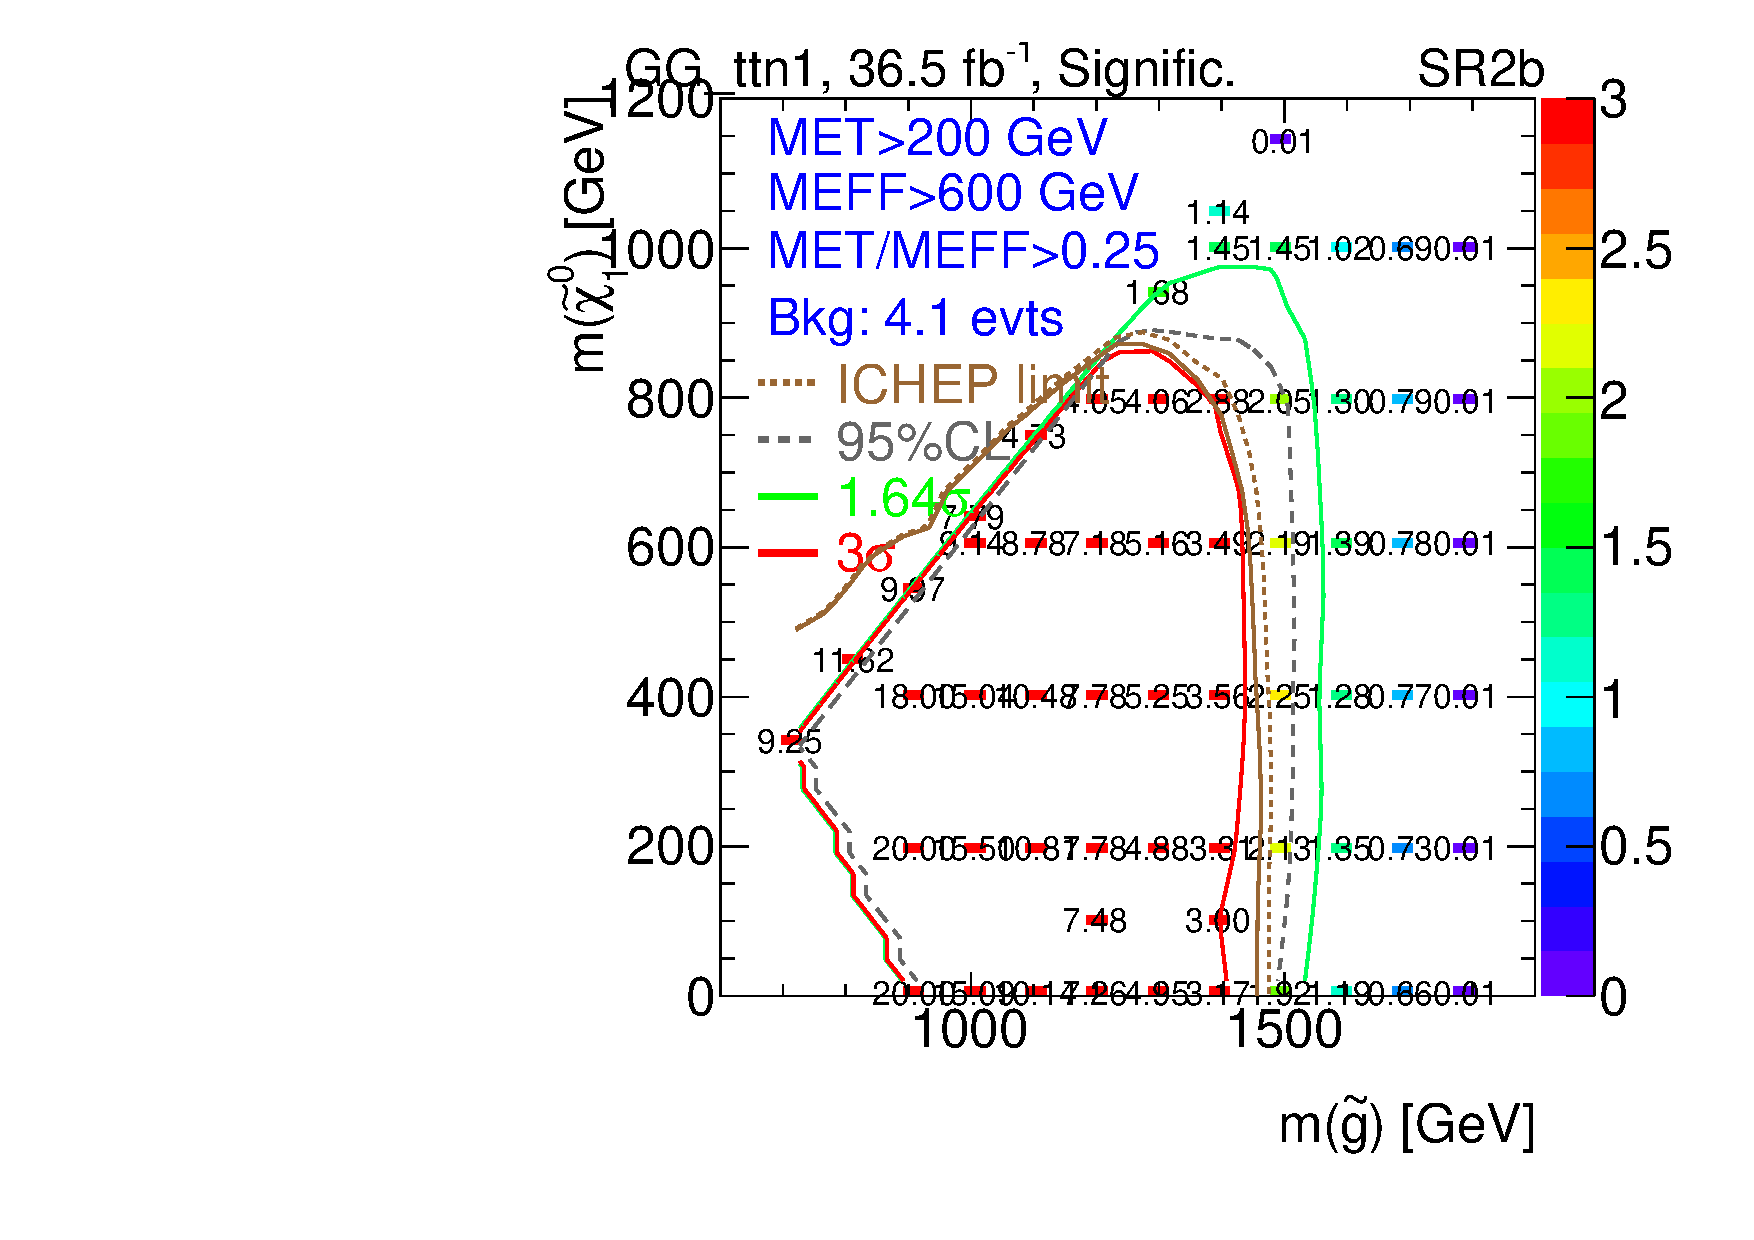
\includegraphics[width=\textwidth,page=1]{2bs.pdf}
\end{subfigure}
\begin{subfigure}[t]{0.48\textwidth}
\caption{Rpc2L2bH}
\includegraphics[width=\textwidth,page=2]{2bs.pdf}
\end{subfigure}
\caption{Discovery significance for the SRs with $b$-jets defined in 
Table~\ref{tab:SRdef3} for 36.5~\ifb: Rpc2L1bS and  Rpc2L1bH in the $\sbot\sbot^*\to t\bar t\tilde\chi_1^+\tilde\chi_1^-$ grid (top), Rpc2L2bS and Rpc2L2bH in the $\gluino\gluino\to t\bar tt\bar t\neut\neut$ grid (bottom). The 95\% CL, 
1.64$\sigma$, and 3$\sigma$ discovery contours from the proposed signal 
regions are shown in grey, green, and red, respectively. 
}
\label{fig:SR_withB}
\end{figure}


\begin{figure}
\centering
\begin{subfigure}[t]{0.48\textwidth}
\caption{Rpc3L0bS}
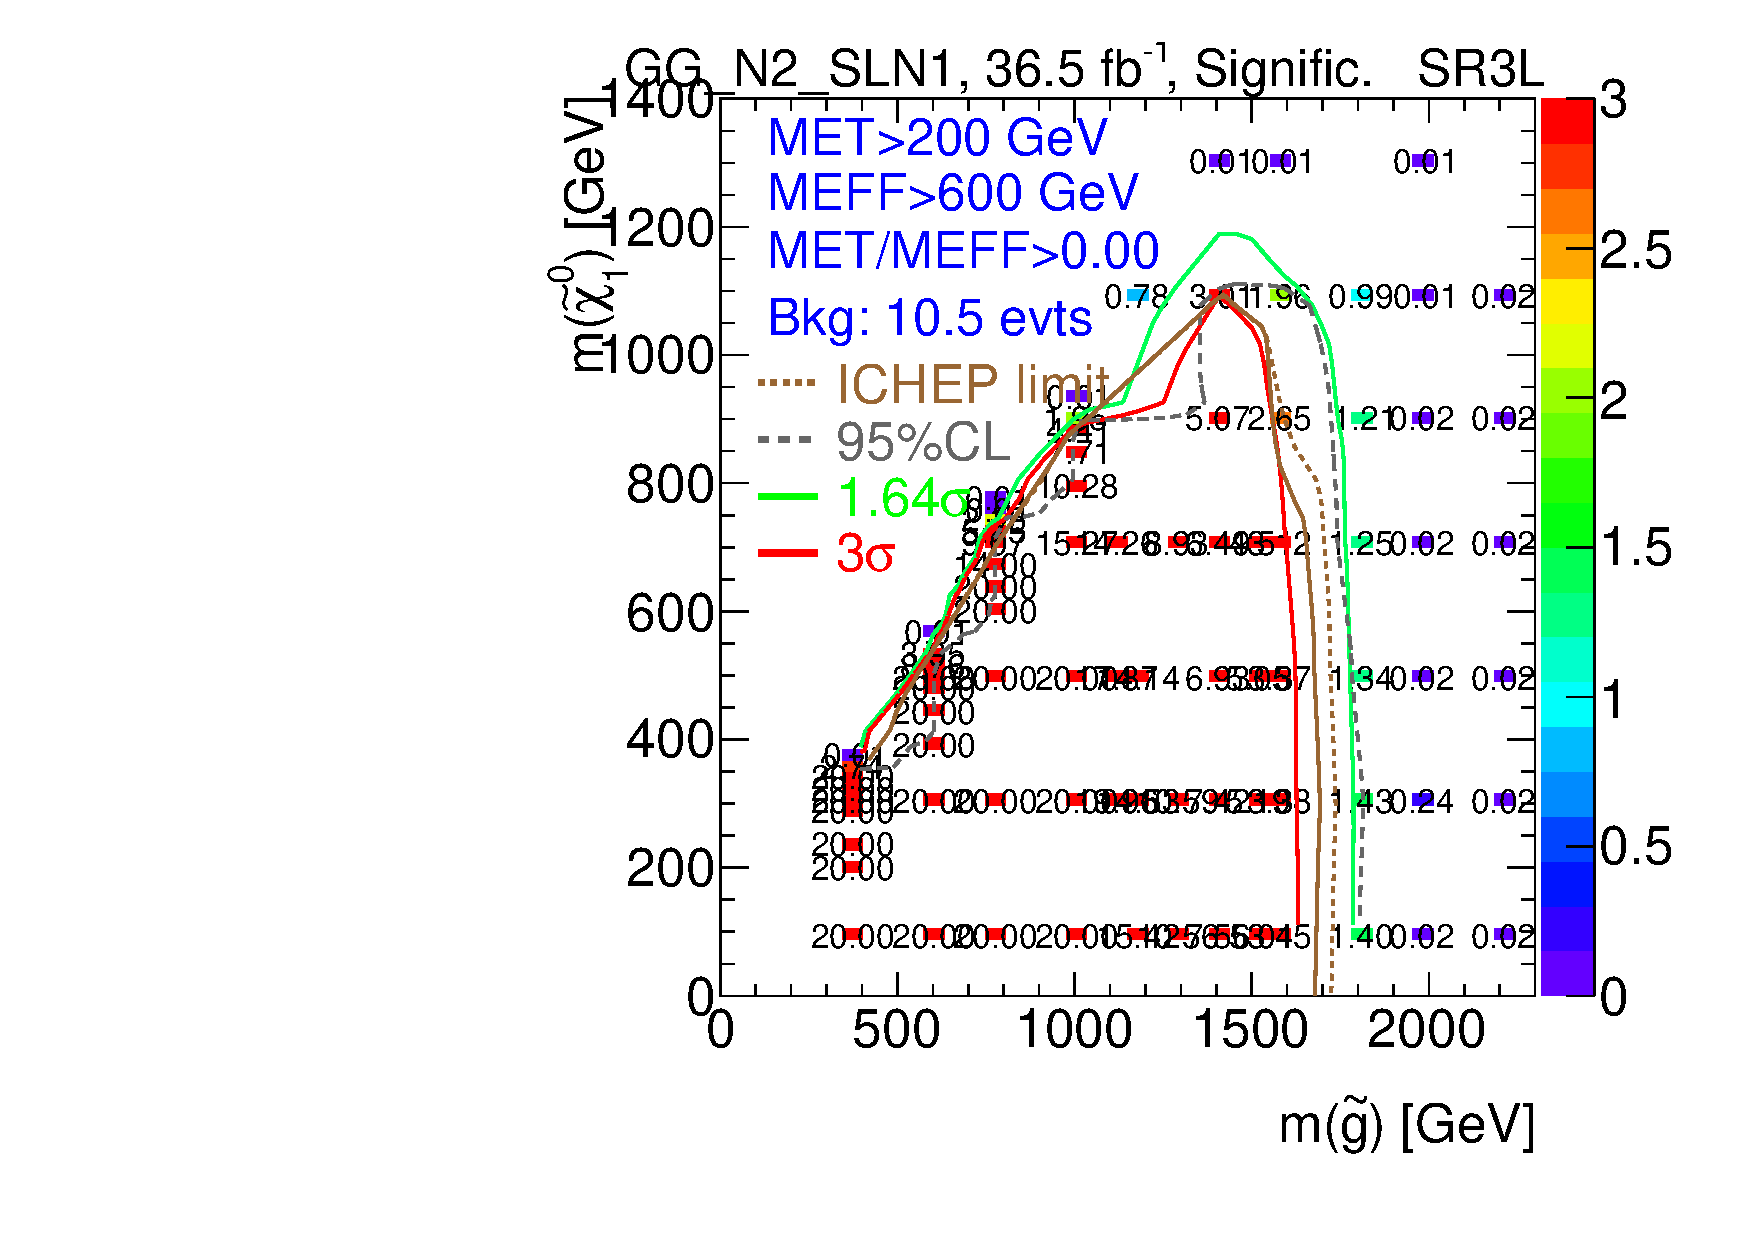
\includegraphics[width=\textwidth,page=1]{allSRs.pdf}
\end{subfigure}
\begin{subfigure}[t]{0.48\textwidth}
\caption{Rpc3L0bH}
\includegraphics[width=\textwidth,page=2]{allSRs.pdf}
\end{subfigure}
\begin{subfigure}[t]{0.48\textwidth}
\caption{Rpc2L0bS}
\includegraphics[width=\textwidth,page=3]{allSRs.pdf}
\end{subfigure}
\begin{subfigure}[t]{0.48\textwidth}
\caption{Rpc2L0bH}
\includegraphics[width=\textwidth,page=4]{allSRs.pdf}
\end{subfigure}
\caption{Discovery significance for the SRs without $b$-jets defined in Table~\ref{tab:SRdef3} for 36.5~\ifb: Rpc2L0bS and Rpc2L0bH in the $\gluino\gluino$ with $\gluino\to q\bar{q}'WZ\neut$ grid (top) and Rpc3L0bS and Rpc3L0bH in the $\gluino\gluino$ with $\gluino\to q\bar{q}(\ell\ell/\ell\nu)\neut$ grid (bottom). The 95\% CL, 1.64$\sigma$, and 3$\sigma$ discovery contours from the proposed signal regions are shown in grey, green, and red, respectively.
}
\label{fig:SR_noB}
\end{figure}


Dedicated new SRs have been optimized for the gluino pair production with stop-mediated decay $\gl\to t\bar t\neut$ with off-shell tops.

The \glgl\ production with $\gl\to t\bar t\neut$ scenario at low LSP masses (where the multi-$b$ analysis has a much better sensitivity
\cite{ATLAS-CONF-2017-021}) is not the only motivation for Rpc2L2bH signal region, but also the NUHM2 model, which features large branching ratios for the $\gluino\to\ttbar\tilde{\chi}_{1,2,3}^0$ and $\gluino\to t\bar{b}\tilde{\chi}_{1,2}^\pm$ decays. As shown in Figure~\ref{fig:SR_nuhm}, with the Rpc2L2bH signal region $m_{1/2}$ values of 600~GeV can be excluded at 95\% CL or observed with a 3$\sigma$ significance.
This SR will be then used for the first interpretation in this model.

\begin{figure}[t]
\centering
\includegraphics[width=0.48\textwidth,page=3]{2bs.pdf}
\caption{Discovery significance for Rpc2L2bH signal region for 36.5~\ifb, NUHM2 model. The 95\% CL, 1.64$\sigma$, and 3$\sigma$ discovery contours from the proposed signal regions are shown in grey, green, and red, respectively.
%: SR0b1 and SR0b2 in the NUHM2
}
\label{fig:SR_nuhm}
\end{figure}


\begin{figure}
\centering
\begin{subfigure}[t]{0.48\textwidth}
\caption{$m_{\gl}$-$m_{\neut}$ mass plane}
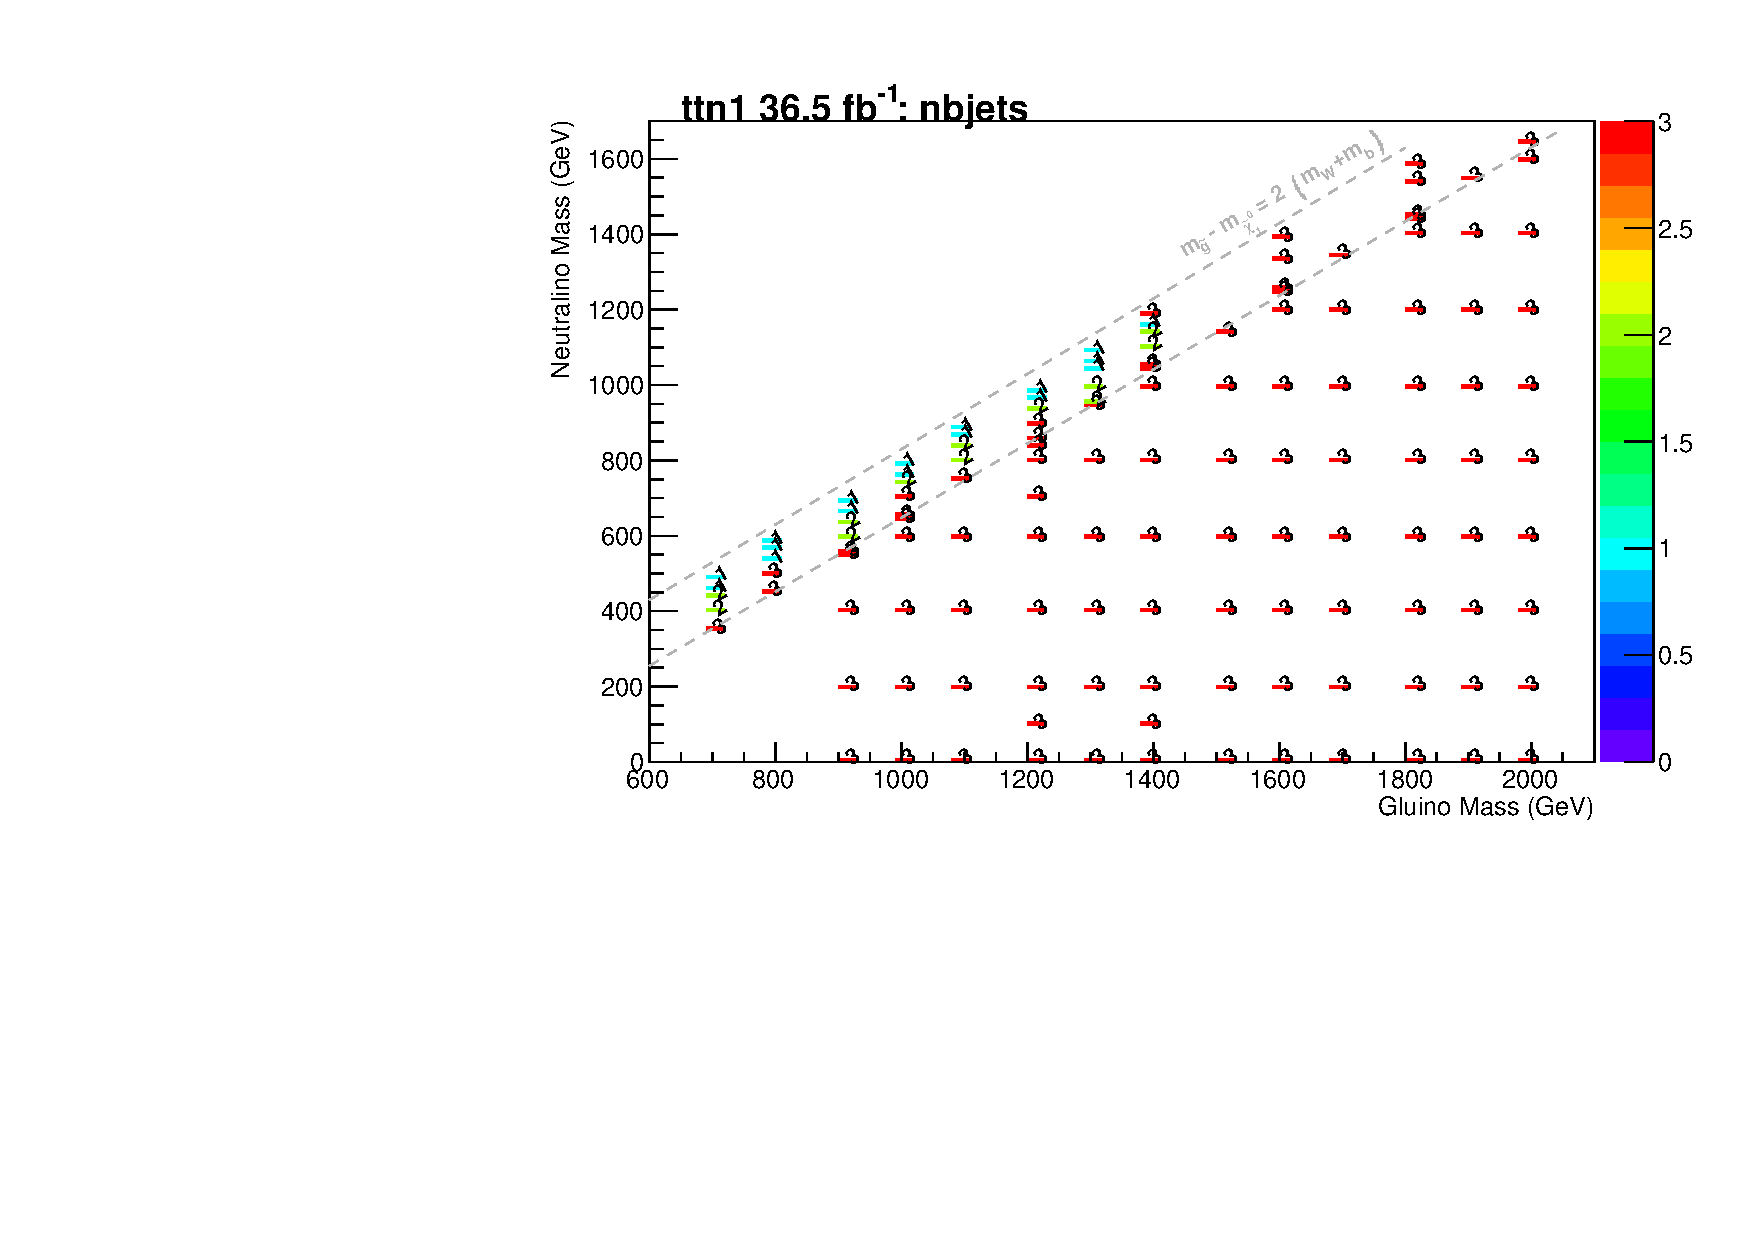
\includegraphics[width=\textwidth]{ttn1_nbjets.pdf}
\end{subfigure}
\begin{subfigure}[t]{0.48\textwidth}
\caption{Above the diagonal}
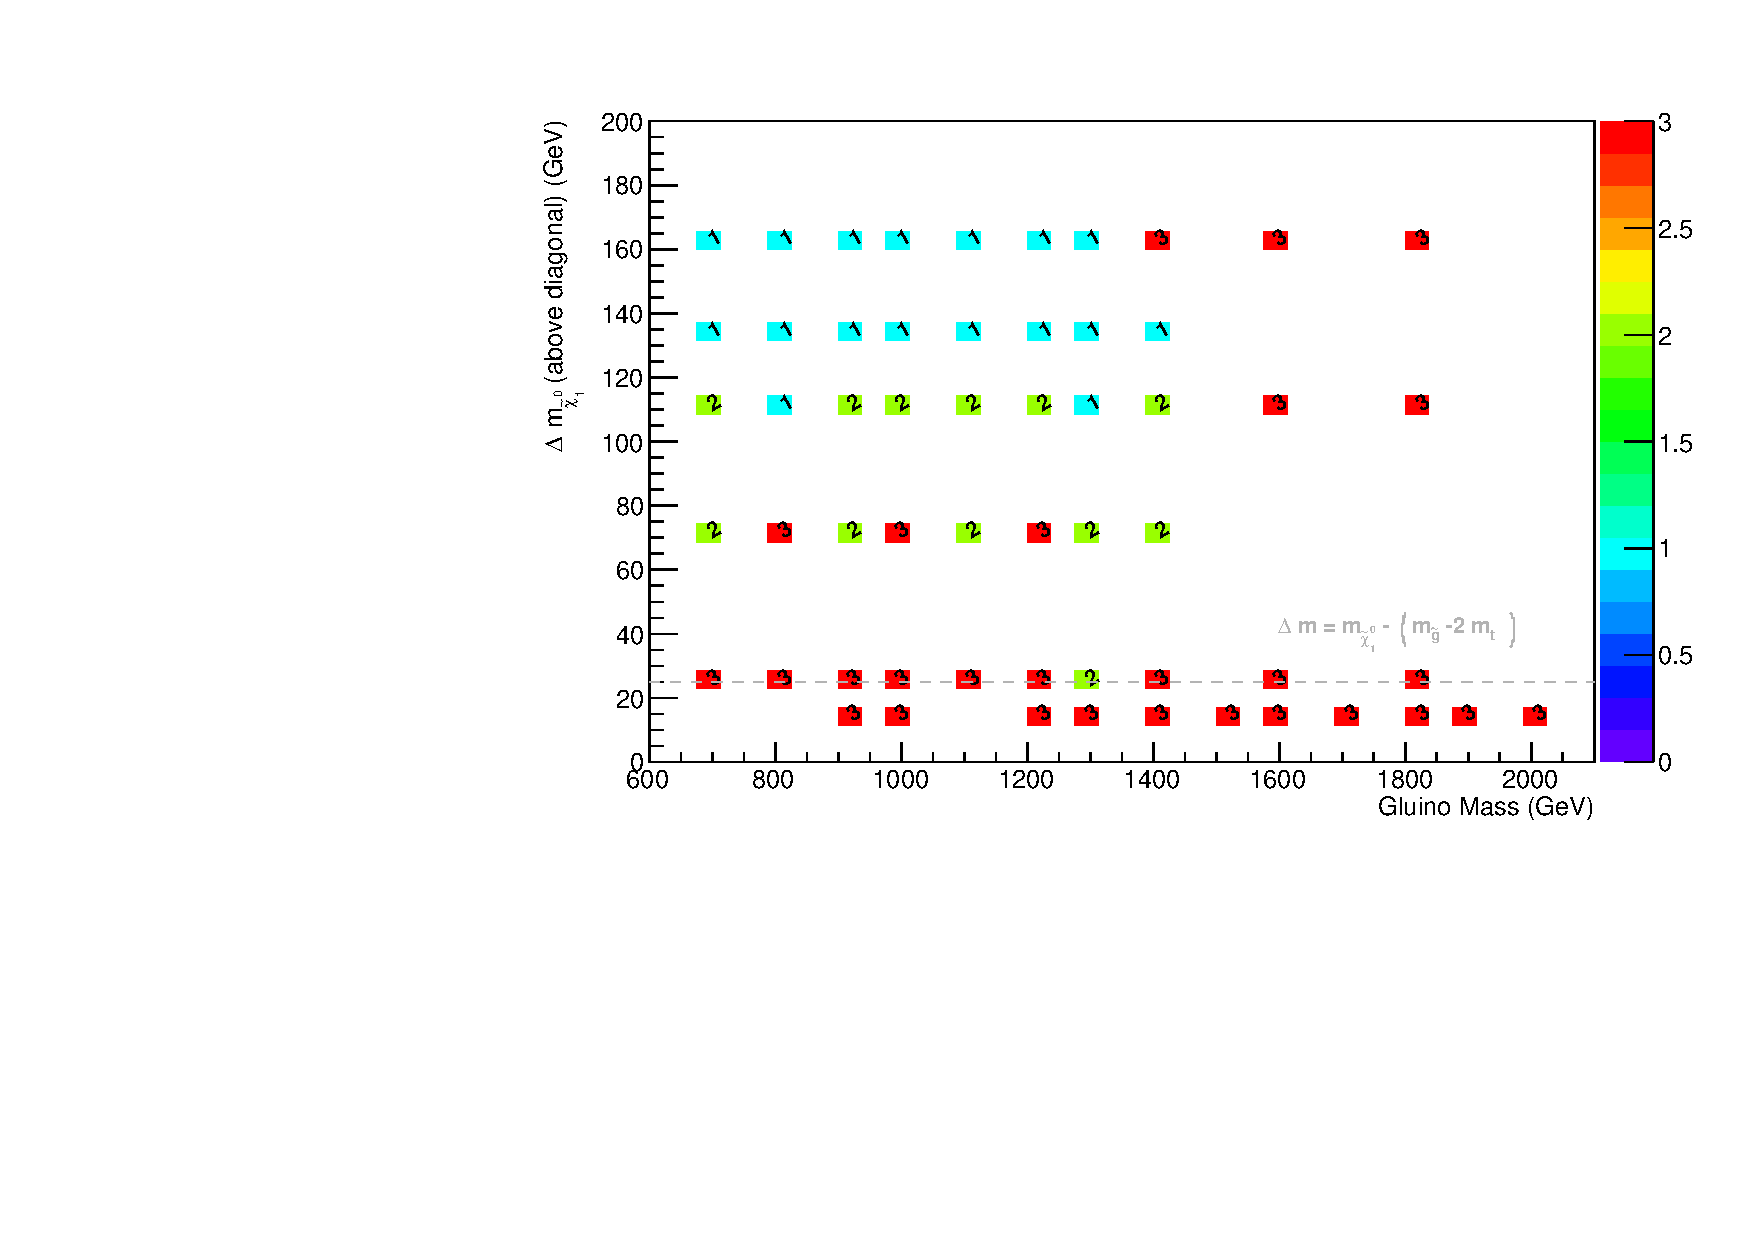
\includegraphics[width=\textwidth]{ttn1_nbjets_Dm.pdf}
\end{subfigure}
\caption{Optimal cut on the number of $b$-jets leading to the best discovery significance.
}
\label{fig:SR_Gtt_bjets}
\end{figure}

\begin{figure}
\centering
\begin{subfigure}[t]{0.48\textwidth}
\caption{Without $p_{\rm T}^{\ell_1}$ uppercut}
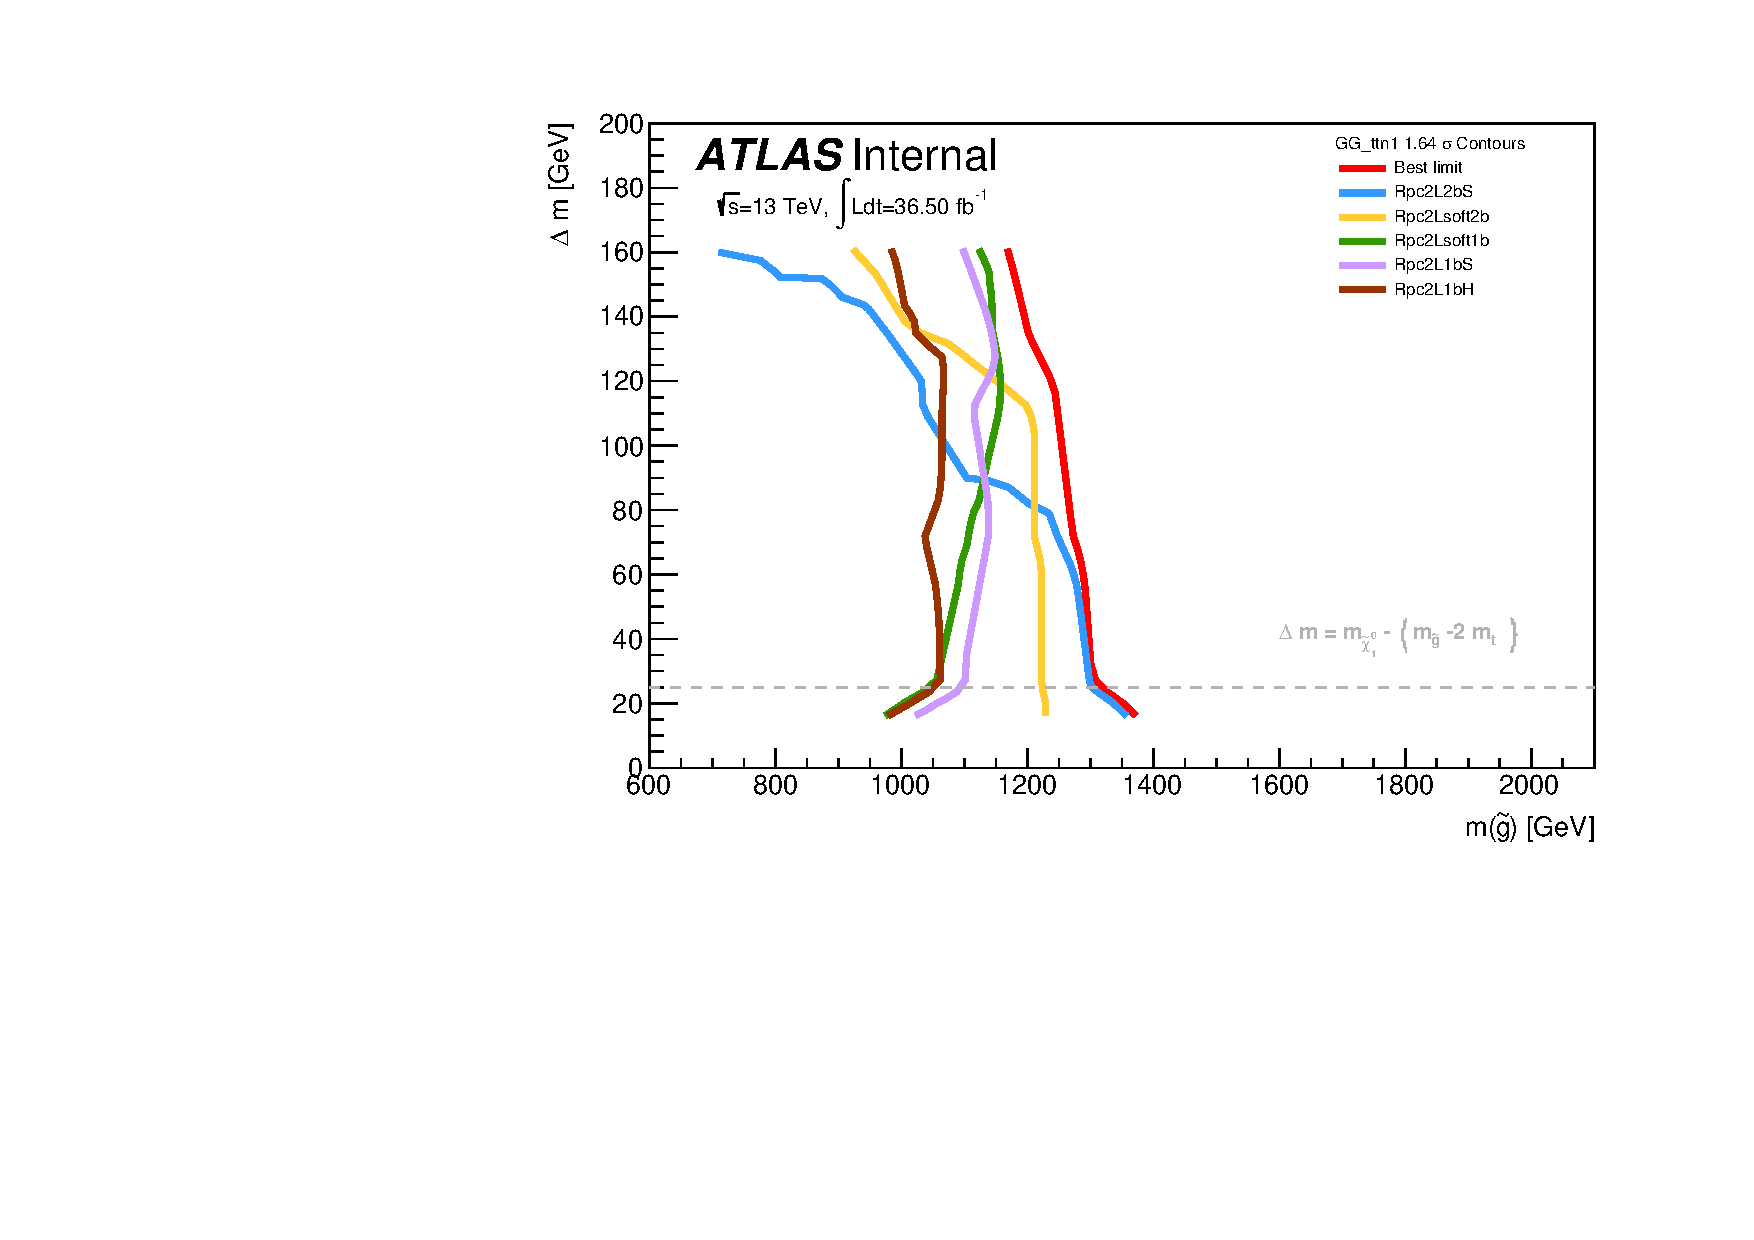
\includegraphics[width=\textwidth]{Gttoff_nobound.pdf}
\end{subfigure}
\begin{subfigure}[t]{0.48\textwidth}
\caption{With $p_{\rm T}^{\ell_1}$ uppercut}
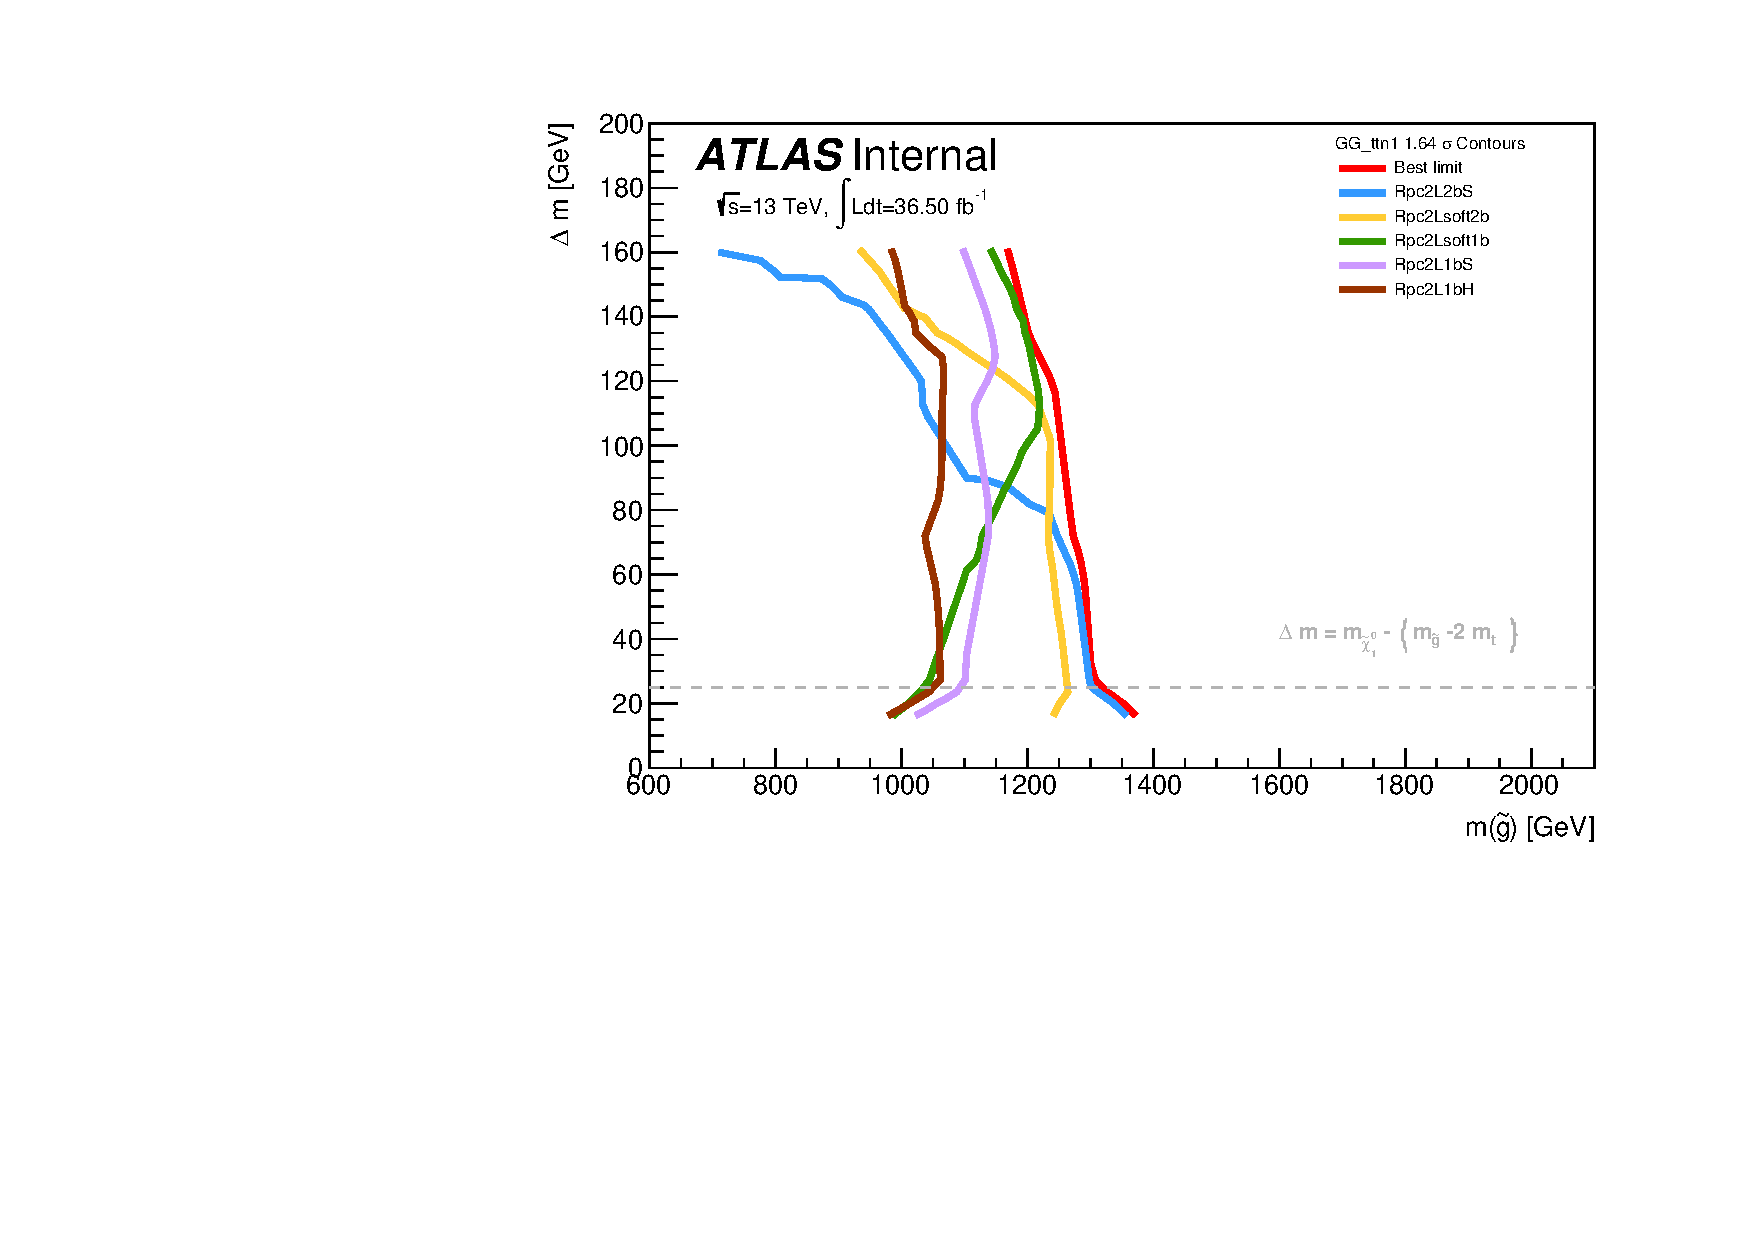
\includegraphics[width=\textwidth]{Gttoff_upbound.pdf}
\end{subfigure}
\caption{Comparison of significance contours at 1.64$\sigma$ for 36.5~\ifb~ between Rpc2Lsoft2b and Rpc2Lsoft1b and other signal regions in the off-diagonal region considering the option of an upper cut on the leading lepton \pt.}
\label{fig:SR_ptbound}
\end{figure}

In addition, the SS/3L analysis has the unique potential to explore the region of phase space at high LSP masses with a more compressed 
spectra. This scenario leads to softer decay products, in particular softer $b$-jets as seen in Figure~\ref{fig:SR_Gtt_bjets}, 
which makes the multi-$b$ analysis less sensitive. For this reason, two additional signal regions were introduced with at least 1 $b$-jet 
(Rpc2Lsoft1b) or 2 $b$-jets (Rpc2Lsoft2b) defined in Table~\ref{tab:SRdef3}. In addition, these signal regions are defined with an upper 
cut on the leading lepton \pt. The sensitivity is degraded if this upper cut is removed as shown in Figure~\ref{fig:SR_ptbound}.

Motivated by the $\stop$ production with $\stopone\to\neuttwo W$ model in Section~\ref{subsec:signals_3lss}, 
the signature of three leptons with the same electric charge (3LSS) is explored for the first time. As shown in Figure~\ref{fig:SR_3lss}, 
after and inclusive 3LSS selection, the background is dominated by dibosons and $Z$+jets (with only one real lepton, and the two other leptons with either an electron with charge mis-identified or a fake lepton) both dominantly without $b$-jets. Once a $b$-jet requirement is applied, the background is dominated by $\ttbar V$, with a clear peak at $m_{\ell\ell}\approx m_Z$ showing that a large fraction of these events are originated from charge mis-identification from events containing $Z\to ee$. After applying a $81<m_{e^\pm e^\pm}<101$~GeV veto, the background is reduced to only 1.7 events for 36.5~\ifb, almost removing the $Z$+jets and diboson backgrounds completely. The final background is dominated by $\ttbar+H,Z,W$, with $\approx$60\% originating from charge flips and $\approx$40\% from fakes and non-prompt leptons. With these very generic selections (Rpc3LSS1b in Table~\ref{tab:SRdef3}), a significance of 3.7$\sigma$ can be obtained for $m_{\stop}=550$~GeV.
Figure~\ref{fig:SR_3lss_final} shows some lepton distributions, including the number of electrons, where most of the charge flip background populates the bins with 2 or 3 electrons, although cutting away those bins would also have a large impact on the signal.

\begin{figure}[htb]
\centering
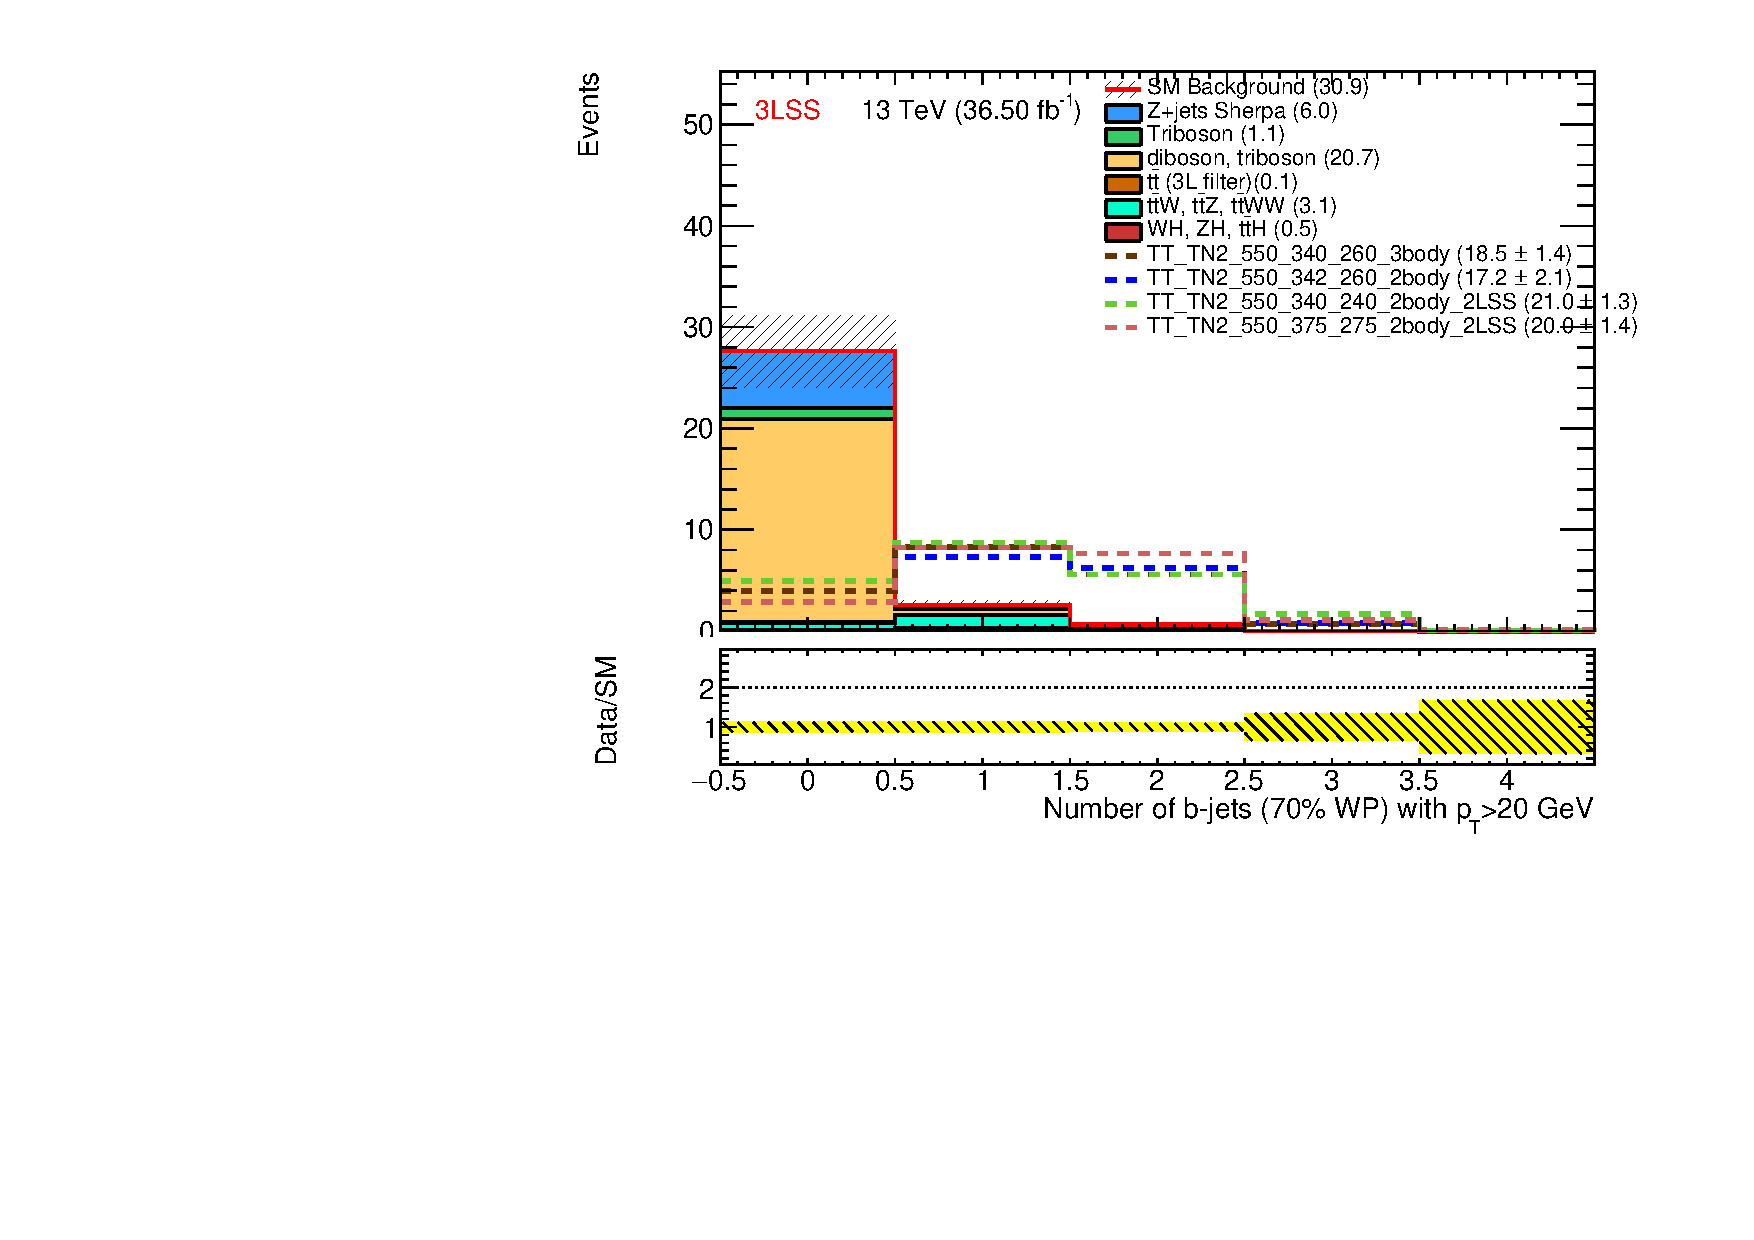
\includegraphics[width=0.45\textwidth]{NBJET70_20_afterlepton_3LSS_0_physics__v47_343637.pdf} 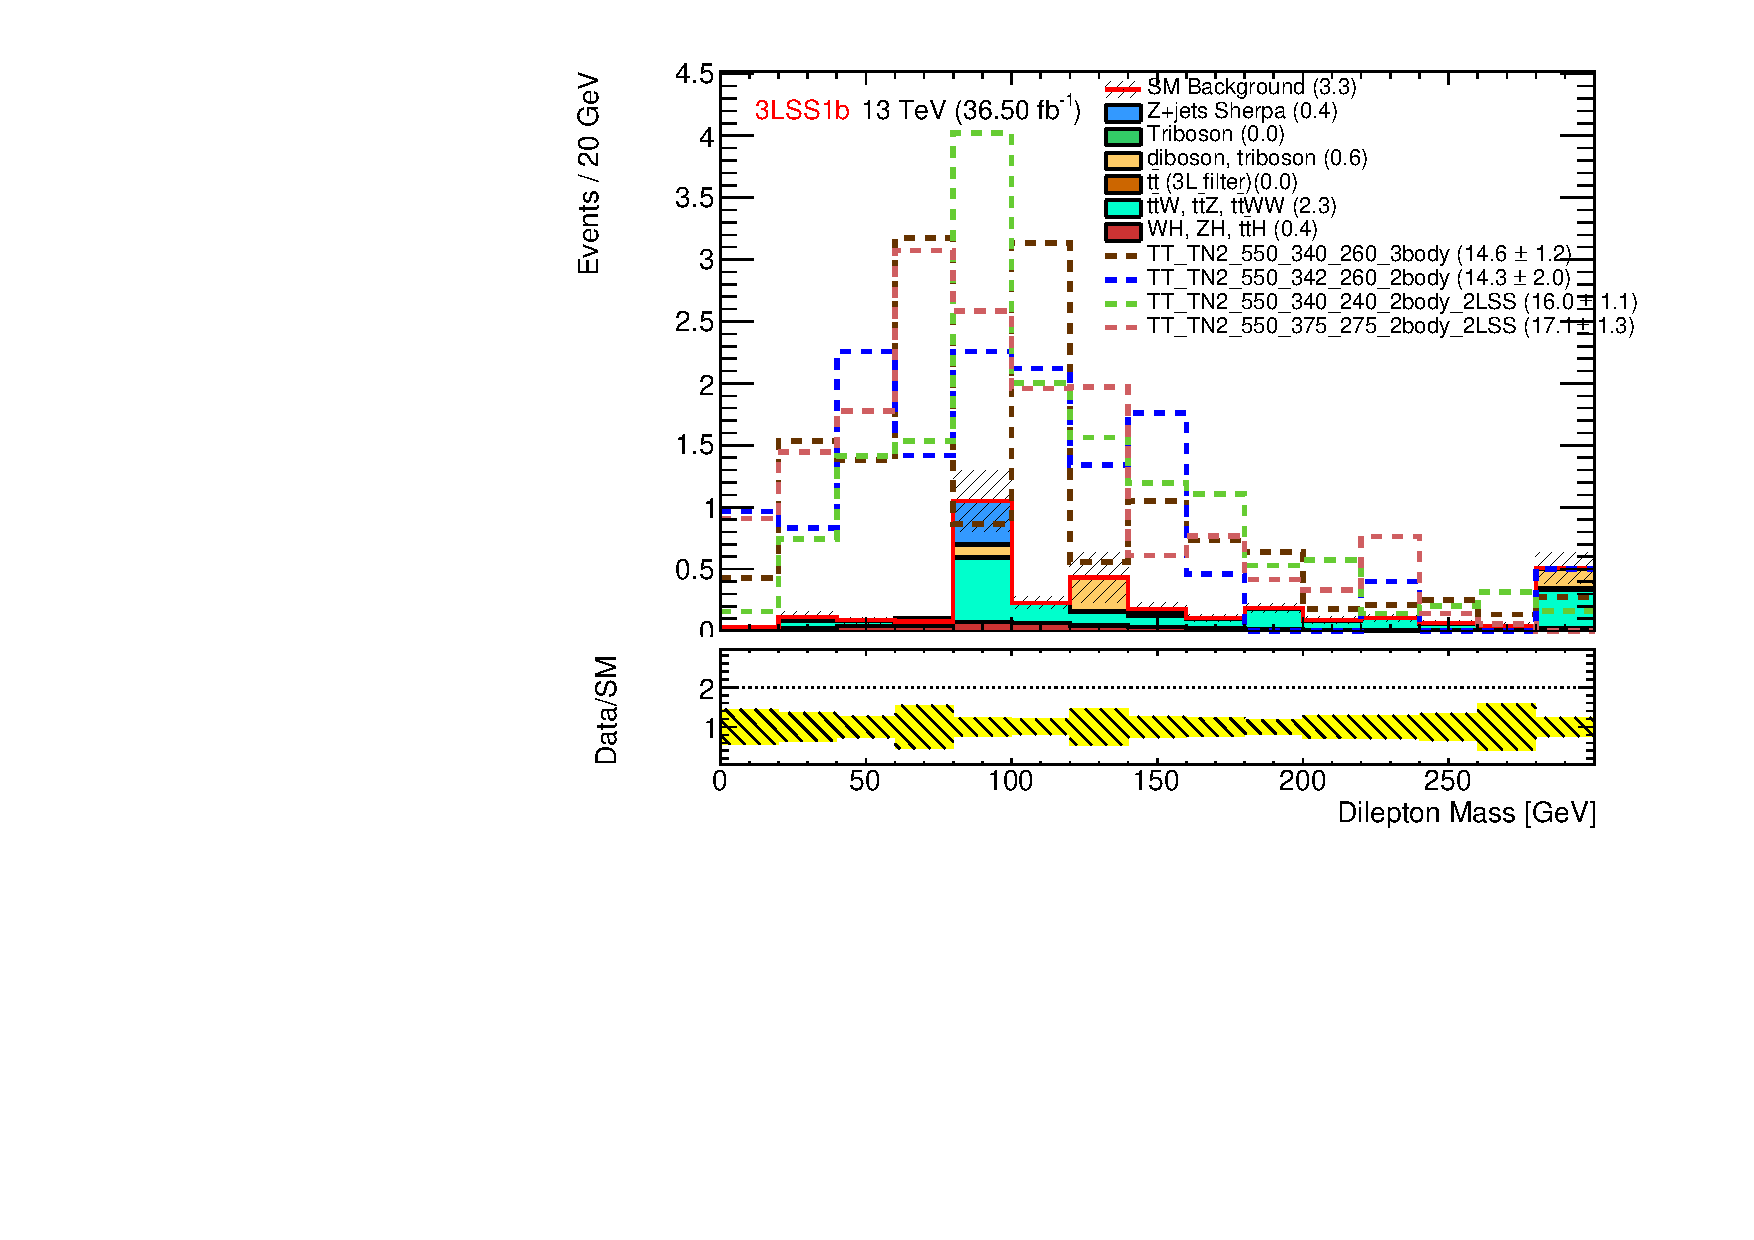
\includegraphics[width=0.45\textwidth]{Mll_afterlepton_3LSS1b_0_physics__v47_343637.pdf} \\
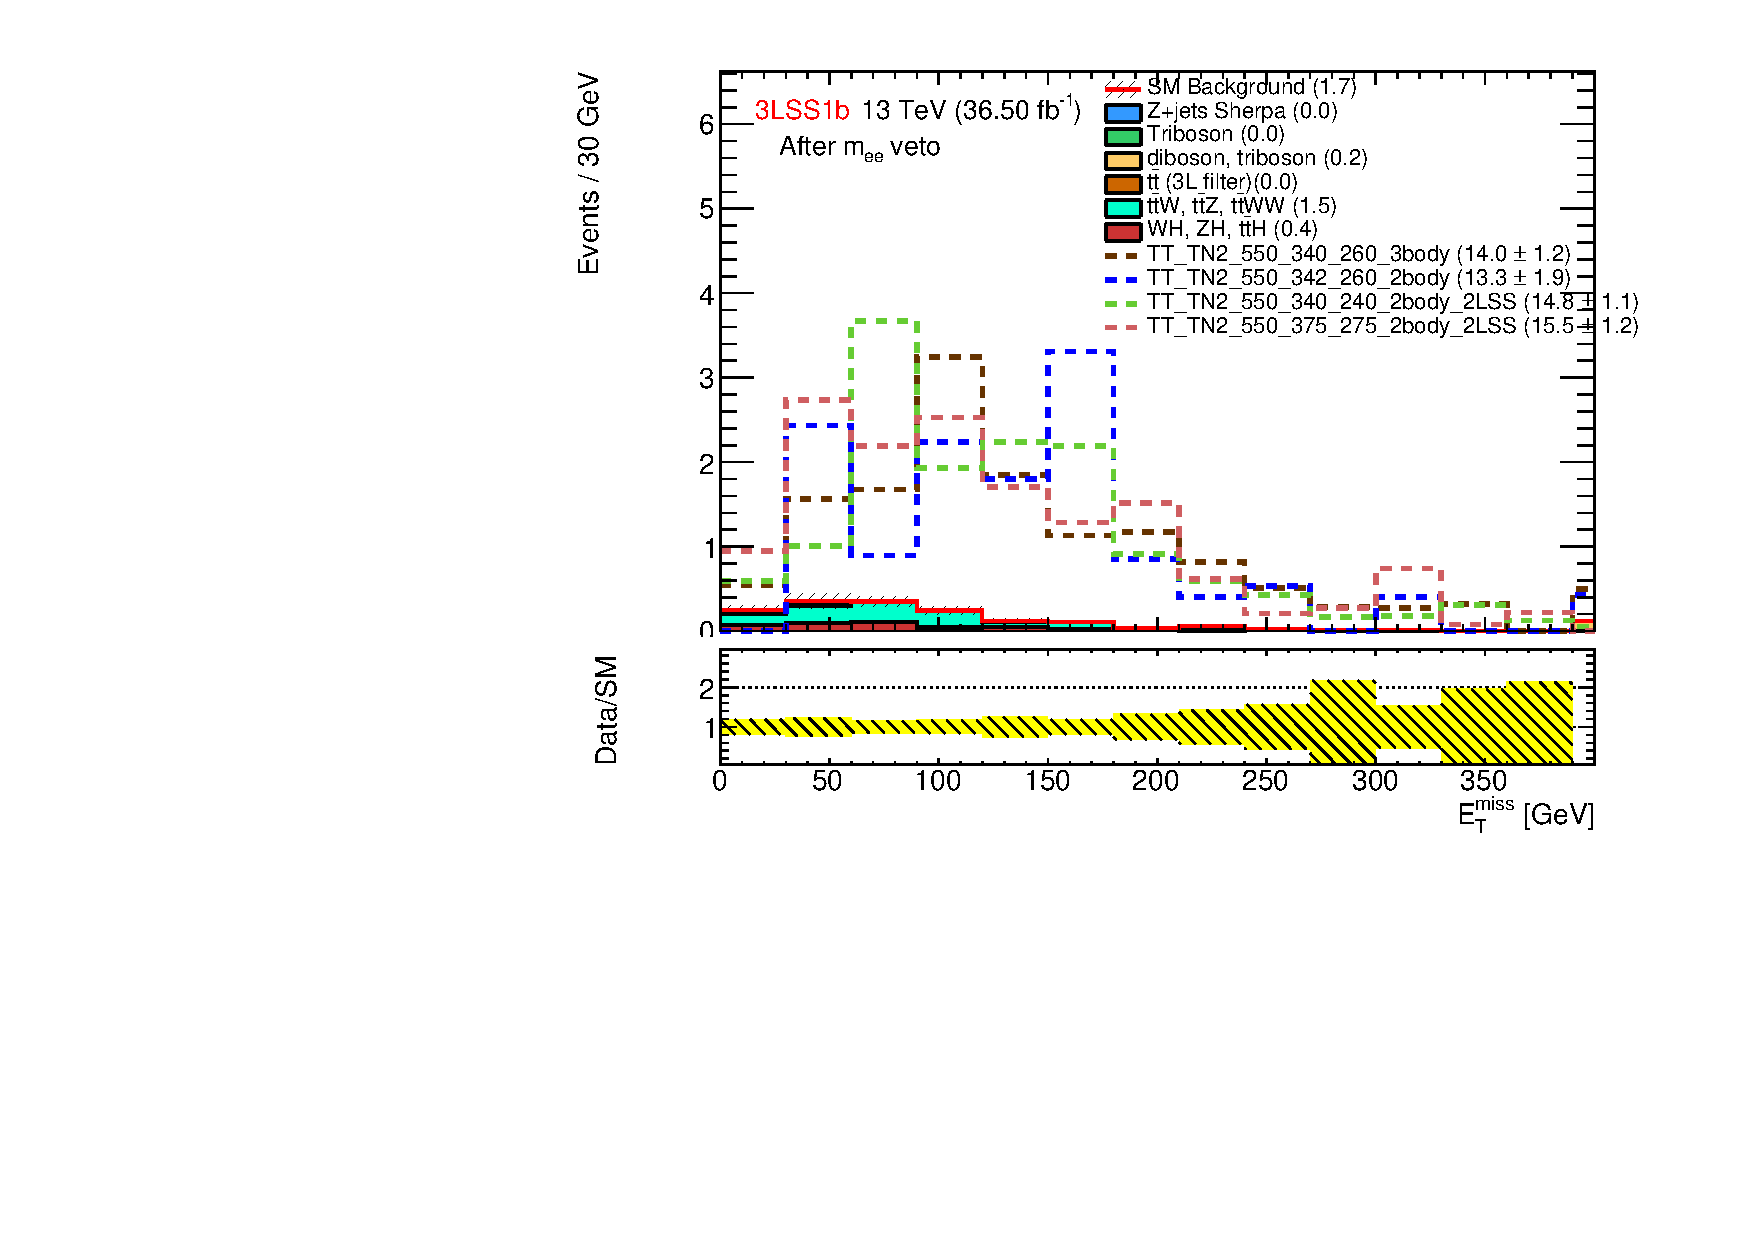
\includegraphics[width=0.45\textwidth]{MET_Mee_3LSS1b_0_physics__v47_343637}
\caption{$b$-jet multiplicity after a 3LSS selection (top left), dilepton invariant mass distributions after a 3LSS plus $\geq$1 $b$-jet selection (top right), and $\met$ distribution after a 3LSS, $\geq$1 $b$-jet and $81<m_{e^\pm e^\pm}<101$~GeV veto selection (bottom), all corresponding to 36.5~\ifb. The background distributions are stacked, while the lines show the predictions for four signal points at $\stop$ mass of 550~GeV.}
\label{fig:SR_3lss}
\end{figure}

\begin{figure}[htb]
\centering
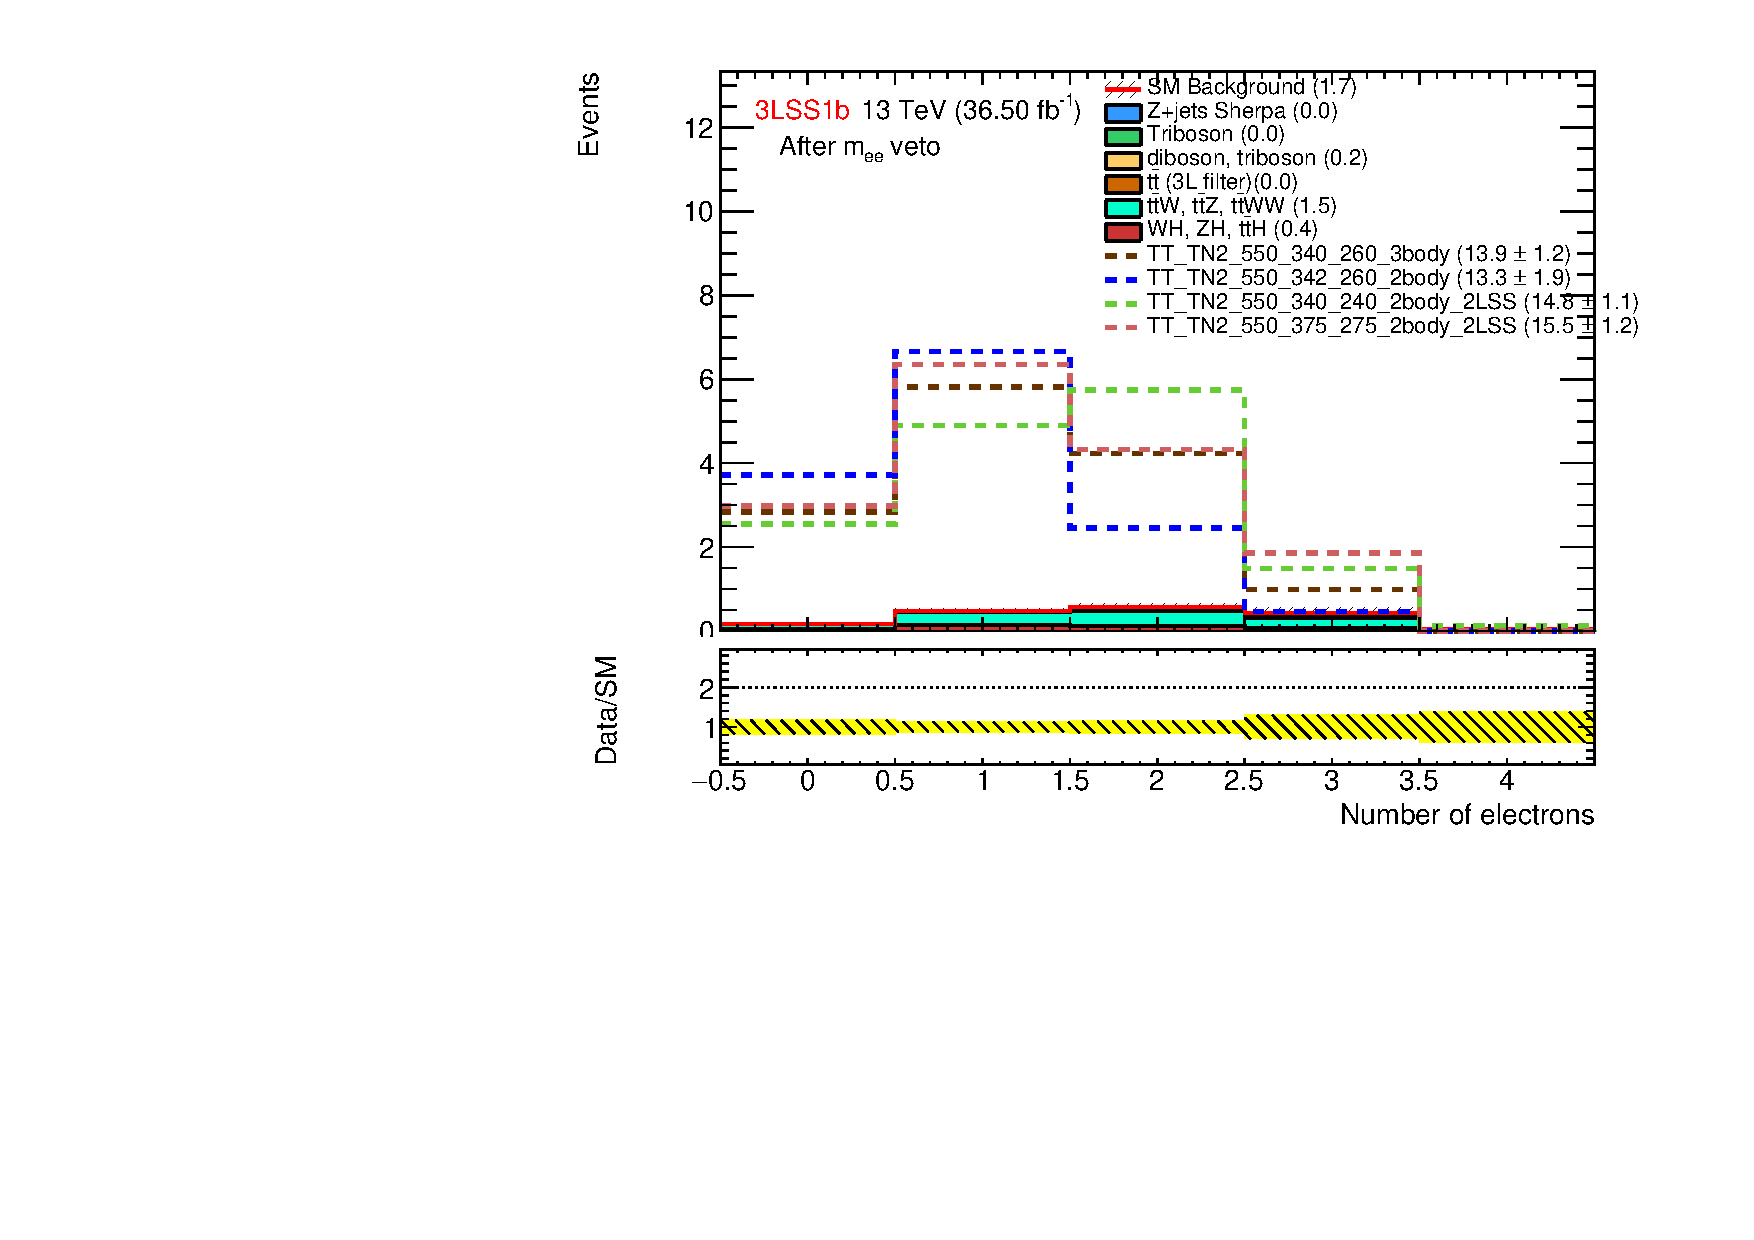
\includegraphics[width=0.45\textwidth]{NEL_Mee_3LSS1b_0_physics__v47_343637.pdf} 
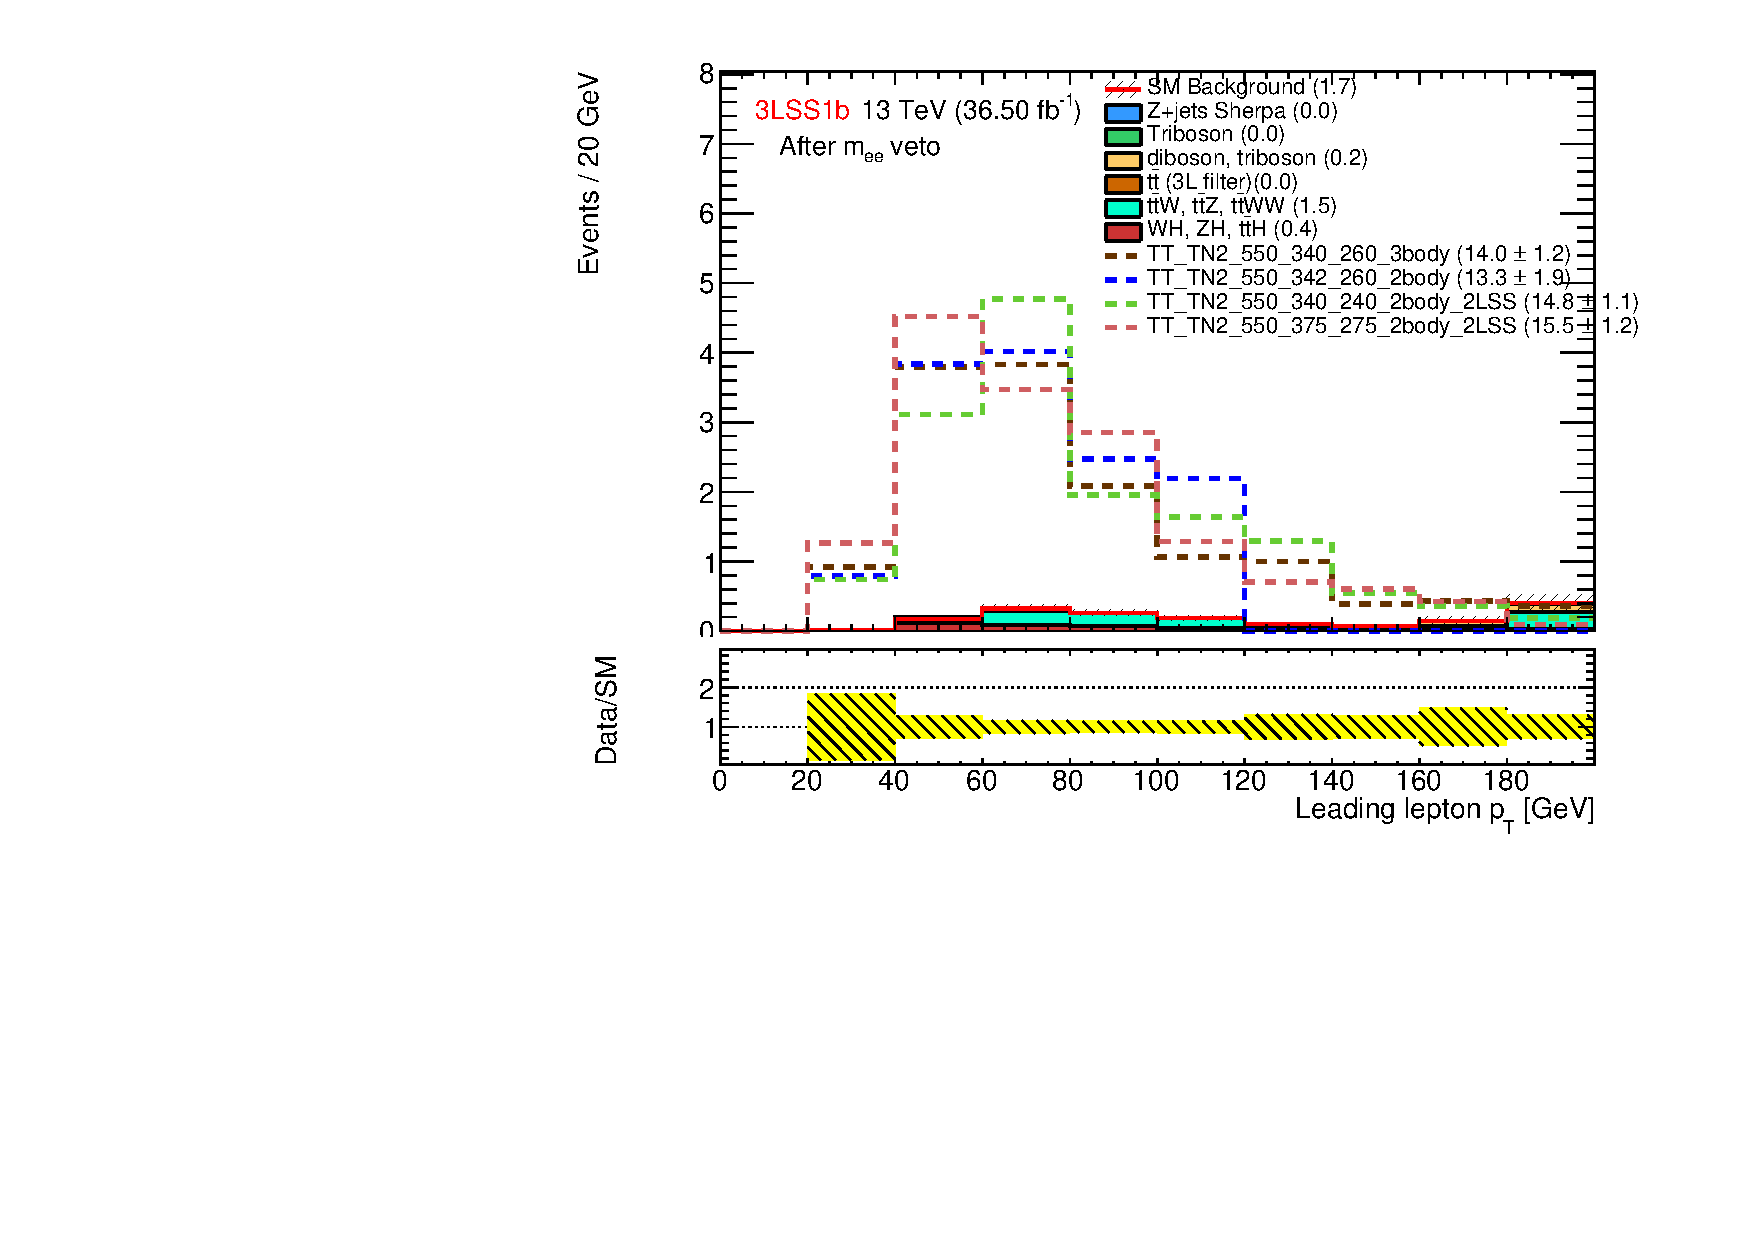
\includegraphics[width=0.45\textwidth]{PTLEP1_Mee_3LSS1b_0_physics__v47_343637.pdf} 
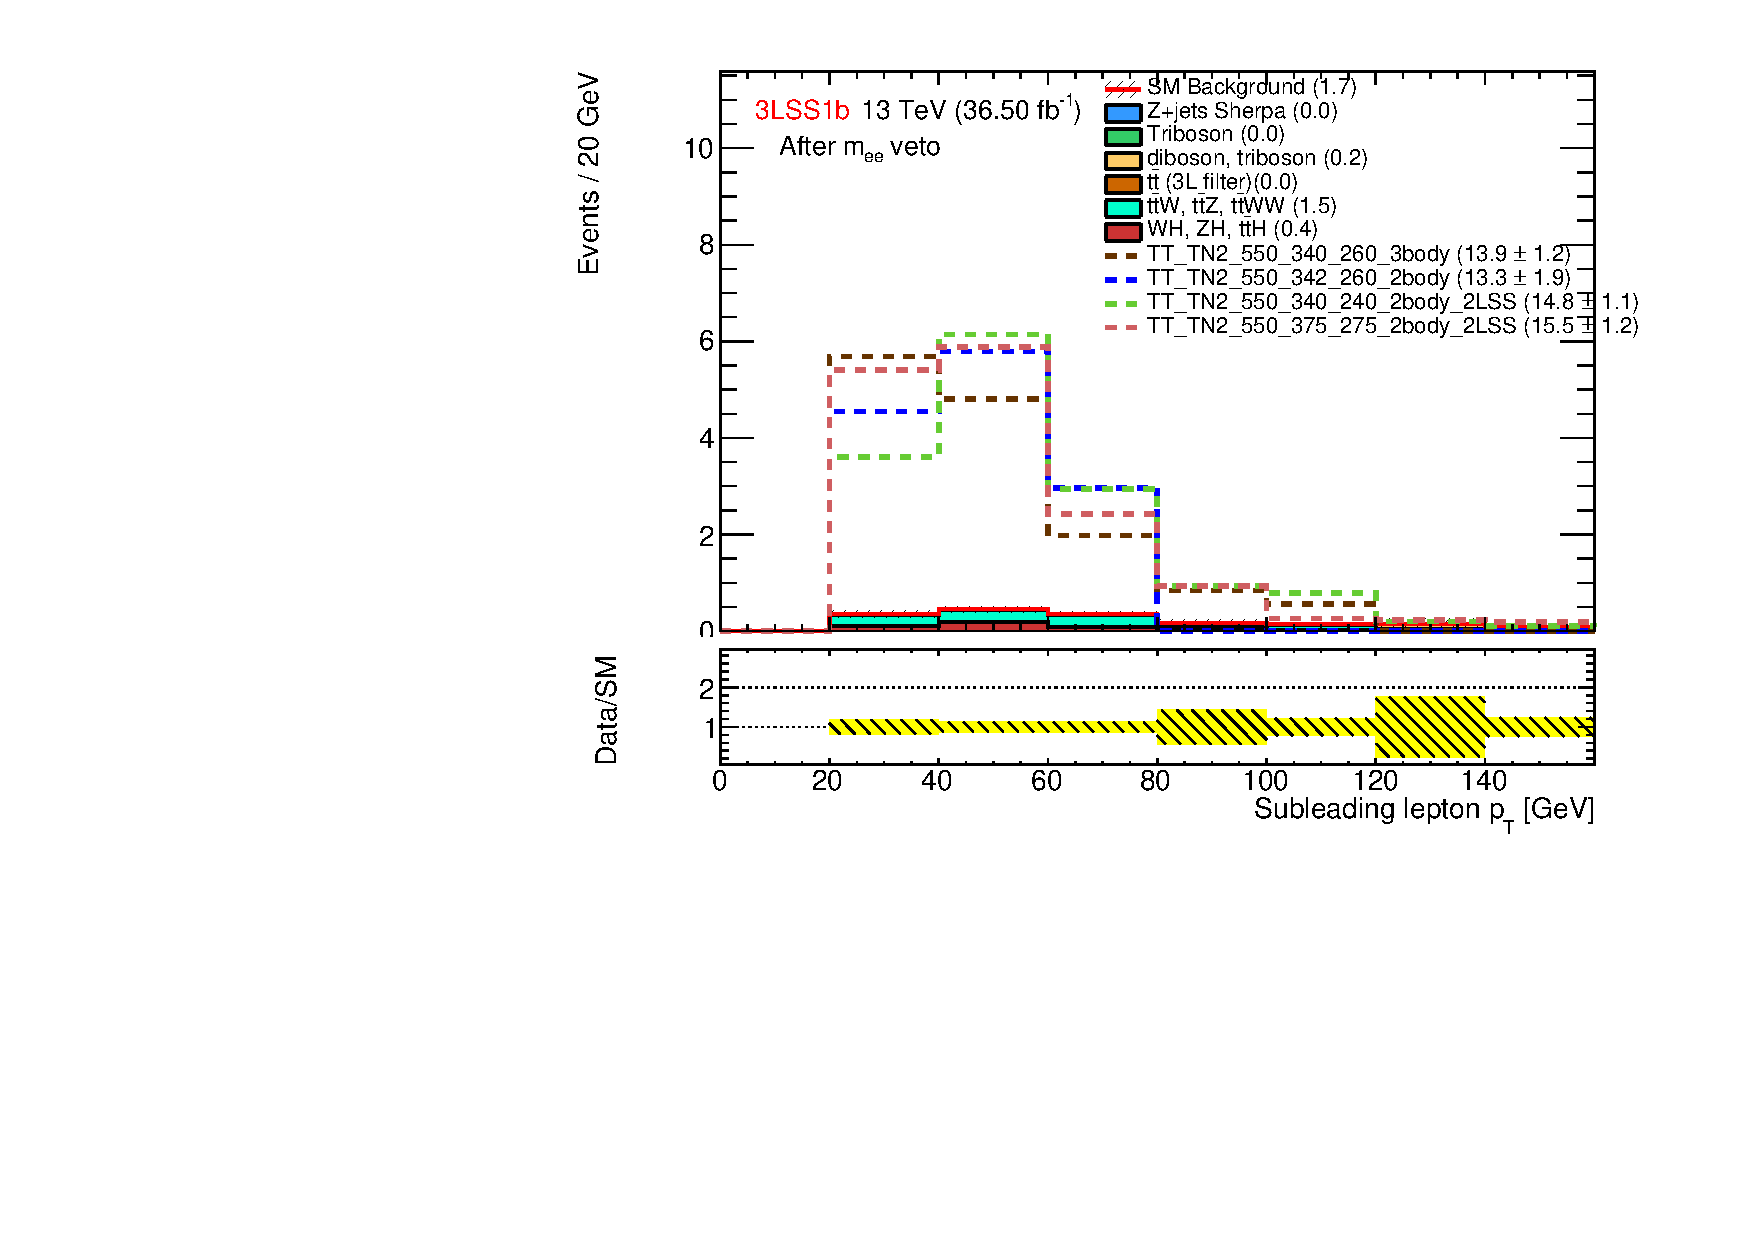
\includegraphics[width=0.45\textwidth]{PTLEP2_Mee_3LSS1b_0_physics__v47_343637.pdf} 
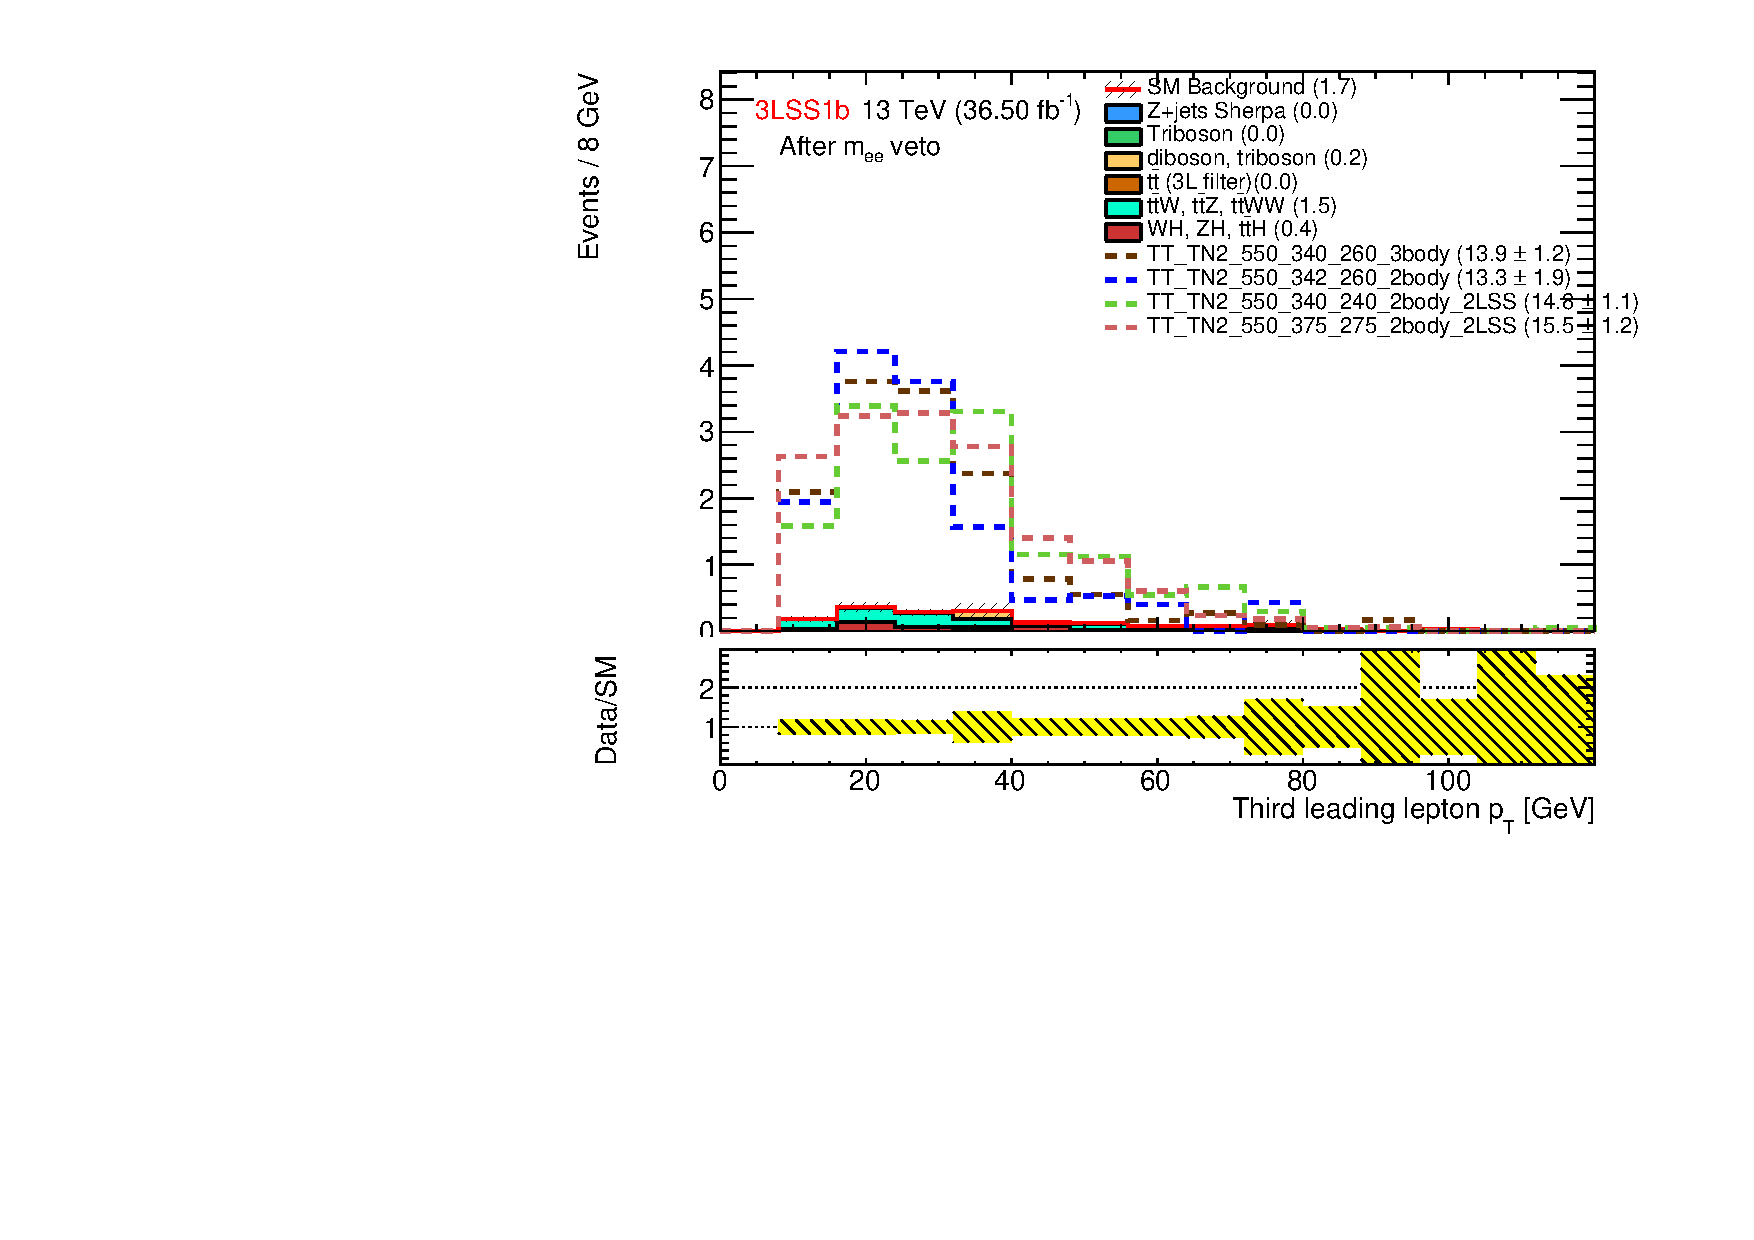
\includegraphics[width=0.45\textwidth]{PTLEP3_Mee_3LSS1b_0_physics__v47_343637.pdf} 
\caption{Number of electron (top left), and $\pT$ of the leading (top right), subleading (bottom left) and third leading lepton (bottom right) after a 3LSS, $\geq$1 $b$-jet and $81<m_{e^\pm e^\pm}<101$~GeV veto selection (bottom), all corresponding to 36.5~\ifb. The background distributions are stacked, while the lines show the predictions for four signal points at $\stop$ mass of 550~GeV.}
\label{fig:SR_3lss_final}
\end{figure}

Finally, since the SRs defined for the \glgl\ production with $\gl\to q\bar q\ell\bar\ell\neut$ feature a $b$-jet veto (Rpc3L0bS and Rpc3L0bH), 
and to avoid leaving uncovered the 3 lepton plus $b$-jets signature, SRs with the same kinematic cuts as Rpc3L0bS and Rpc3L0bH but with a $\geq$1 $b$-jet requirement are also proposed in Table~\ref{tab:SRdef3} as Rpc3L1bS and Rpc3L1bH. 
